\documentclass[11pt]{article}
\usepackage[a4paper,margin=2.5cm]{geometry}
\usepackage{amsmath,amssymb,amsthm,mathtools}
\usepackage{booktabs,enumitem,xcolor,graphicx,array}
\usepackage{algorithm}
\usepackage{algpseudocode}
\usepackage{tikz}
\usetikzlibrary{arrows.meta,positioning,calc}
\usepackage{pgfplots}
\pgfplotsset{compat=1.17}
\usepgfplotslibrary{fillbetween,groupplots}
\usepackage{hyperref}
\hypersetup{colorlinks=true,linkcolor=blue!50!black,citecolor=blue!50!black,urlcolor=blue!50!black}

\newtheorem{theorem}{Theorem}
\newtheorem{lemma}[theorem]{Lemma}
\newtheorem{proposition}[theorem]{Proposition}
\newtheorem{corollary}[theorem]{Corollary}
\theoremstyle{definition}
\newtheorem{definition}[theorem]{Definition}
\newtheorem{assumption}{Assumption}
\renewcommand{\theassumption}{A\arabic{assumption}}
\theoremstyle{remark}
\newtheorem{remark}[theorem]{Remark}
\newtheorem{example}[theorem]{Example}

\newcommand{\E}{\mathbb{E}}
\newcommand{\Prob}{\mathbb{P}}
\newcommand{\KL}{\mathrm{KL}}
\newcommand{\kl}{\mathrm{kl}}
\newcommand{\err}{\mathrm{err}}
\newcommand{\Qt}{\widetilde{Q}}
\newcommand{\Pt}{\widetilde{P}}
\newcommand{\Z}{\mathbb{Z}}
\newcommand{\R}{\mathbb{R}}
\newcommand{\dd}{\mathrm{d}}
\newcommand{\rint}{\operatorname{rint}}
\newcommand{\review}[1]{\par\smallskip\noindent\fcolorbox{red!50!black}{red!3}{\parbox{0.96\linewidth}{\small\textbf{To check.} #1}}\par\smallskip}
\newcommand{\intuition}[1]{\par\smallskip\noindent\fcolorbox{blue!40!black}{blue!3}{\parbox{0.96\linewidth}{\small\textbf{Intuition.} #1}}\par\smallskip}

\title{Certifying the network a sampler outputs:\\ a prequential PAC-Bayes bound from data-tempered annealing,\\ with an exact implementation}
\author{Working draft for internal review (written with Claude; every claim to be checked)}
\date{21 November 2026}

\begin{document}
\maketitle

\begin{abstract}
PAC-Bayes certificates for neural networks with data-free priors are usually loose because the posterior must be a
simple family, typically a Gaussian placed around an SGD solution, and its divergence from the prior grows with the
distance the weights travelled. The posterior that would minimise the bound, the Gibbs (tempered Bayesian) posterior,
has a divergence that is small whenever the model predicts new points well after seeing few examples; but that
divergence involves an intractable marginal likelihood, and we cannot sample the posterior exactly. We show that one
can certify \emph{the network actually produced} by a Markov chain that starts at the prior and absorbs the training set
block by block, with each block scored before the chain uses it. The complexity term is the exact log-density ratio
between the whole run and a time-reversed run started at the prior. It equals $\lambda$ times the area under the run's
online log-loss curve minus its final training loss, and it needs no mixing assumption and no estimated expectation.
We extend the bound to particle methods, explain why floating-point implementations violate its hypotheses in a way
that no small correction repairs, and give an exact implementation on integer lattices. With data-free scattering
features we obtain certificates of $0.060$ on MNIST, $0.217$ on Fashion-MNIST and $0.612$ on CIFAR-10 (full training
sets, ten classes, $\delta=0.025$).
\end{abstract}

\tableofcontents
\newpage

%======================================================================
\section{Motivation}\label{sec:motivation}

\paragraph{The question.} A trained network has small error on its training set. A \emph{generalisation certificate}
is a number, computed from the training set alone, that upper-bounds the network's error on new data with high
probability. Certificates matter in practice (a guarantee without held-out data) and as explanations: a tight
certificate identifies a quantity that actually accounts for why the network generalises. For deep networks with priors
that do not look at the data, the best published certificates are around $0.12$--$0.3$ on MNIST, against test errors of
$1$--$3\%$, and around $0.72$ on CIFAR-10.

\paragraph{Why PAC-Bayes certificates are loose.} A PAC-Bayes bound (Section~\ref{sec:pacbayes}) charges the
Kullback--Leibler divergence $\KL(Q\|P)$ between a \emph{posterior} $Q$ (a distribution over networks chosen after
seeing the data) and a \emph{prior} $P$ (chosen before). The standard recipe (Dziugaite and Roy, 2017; P\'erez-Ortiz et
al., 2021) takes $P$ Gaussian around the initialisation and $Q$ Gaussian around the trained weights. Two things then go
wrong. The KL grows with the squared distance between the two centres, and SGD moves weights a long way. And a Gaussian
is a poor shape for the set of good networks, so $Q$ must stay narrow and pays for that precision too.

\paragraph{What the ideal posterior pays.} For a fixed trade-off between fit and complexity, the posterior that
minimises the PAC-Bayes objective is the \emph{Gibbs posterior} $\pi_\lambda(\dd w)\propto e^{-\lambda L(w)}P(\dd w)$,
where $L$ is the summed training loss (Catoni, 2007). With the cross-entropy loss and $\lambda=1$ it is the Bayesian
posterior. Its divergence from the prior can be read off an online learning curve (Section~\ref{sec:prequential}):
\[
\KL(\pi_\lambda\|P)\ \approx\ \lambda\Big[\underbrace{\textstyle\sum_{i=1}^n \text{loss on $z_i$ predicted from $z_1,\dots,z_{i-1}$}}_{\text{prequential loss}}\ -\ \underbrace{\text{final training loss}}_{\text{fit}}\Big]
\]
(Proposition~\ref{prop:intuition} makes this precise). A model that predicts the $i$-th example well after seeing
$i-1$ examples is cheap. This is the Bayesian and
minimum-description-length view of generalisation (Dawid, 1984; Blier and Ollivier, 2018; Lyle et al., 2020): models
generalise when they learn quickly. It is also what one would like a certificate to measure.

\paragraph{Why it is not directly usable.} The identity involves the marginal likelihood (the normaliser of
$\pi_\lambda$), which is intractable for a network, and it is about $\pi_\lambda$ itself, which we cannot sample exactly.
Annealed importance sampling (AIS; Neal, 2001) gives an unbiased \emph{estimate} of the marginal likelihood, but an
estimate is not a certificate, and the network that AIS returns is not an exact posterior sample.

\paragraph{The idea of this note.} Certify the network the sampler \emph{actually returns}, and compare the whole run,
not just its output, with a reference process. Run a Markov chain that starts from the prior and absorbs the training
set block by block, moving at each stage with an MCMC kernel that leaves the current partial posterior invariant.
Compare this run with the time-reversed run that starts from the prior at the final time (Figure~\ref{fig:paths}); this
reference is an imaginary process used only in the analysis, never simulated. The
log-density ratio between the two path distributions can be computed exactly on the realised run, and it turns out to
be the prequential quantity above: $\lambda$ times the online loss of the run (each block scored before the chain has
used it) minus the final training loss. PAC-Bayes on path space then gives a certificate for the single output network.
Nothing needs to mix; poor mixing only makes the certificate looser.

\paragraph{Exactness.} A certificate is a statement about exact probability ratios. Floating-point MCMC breaks those
ratios in a way that no small correction repairs (Section~\ref{sec:exact}), as is known for differential privacy
(Mironov, 2012). We therefore also give an implementation on integer lattices with exact discrete sampling, for which the
hypotheses hold bit for bit.

\paragraph{Contributions.}
\begin{enumerate}[nosep]
\item A disintegrated PAC-Bayes certificate for the output of an annealed MCMC run, whose complexity is the realised
  log-ratio between the run and a time-reversed reference run (Theorem~\ref{thm:cert}). The reference depends on the
  training set, which a PAC-Bayes prior may not, but only its data-free marginal at the output enters.
\item A data path that charges each training point once, when it arrives, so the complexity is a prequential code
  length; a decomposition showing it upper-bounds the ideal Gibbs-posterior KL by per-block Jensen gaps
  (Proposition~\ref{prop:intuition}); and the extension to particle methods.
\item An exact (floating-point-free) implementation, and validity tests that catch the likely mistakes.
\item Data-free certificates of $0.060$ (MNIST), $0.217$ (Fashion-MNIST) and $0.612$ (CIFAR-10).
\end{enumerate}

\subsection{How this relates to what you may know}\label{sec:glance}
Table~\ref{tab:glance} places the method among existing approaches. In short: it is PAC-Bayes with the best-shaped
posterior (a tempered Bayesian posterior over the network, approximated by MCMC), made computable by moving the
comparison to path space, where AIS's importance weight is an exact density ratio rather than an estimate.

\begin{table}[t]
\centering\small
\renewcommand{\arraystretch}{1.25}
\begin{tabular}{@{}p{3.5cm}p{3.3cm}p{3.9cm}p{4.0cm}@{}}
\toprule
approach & what is certified & what is paid (complexity) & main limitation\\
\midrule
Gaussian PAC-Bayes (Dziugaite \& Roy 2017; P\'erez-Ortiz et al.\ 2021) & a random network drawn from a Gaussian around SGD weights & KL between two Gaussians: distance from initialisation & posterior shape; distance travelled by SGD\\
Compression (Lotfi et al.\ 2022) & the compressed network & description length of the compressed weights & compression must preserve accuracy\\
Priors from private training (Dziugaite \& Roy 2018; Lampert et al.\ 2026) & a network trained by noisy SGD & information leaked by the noisy training & the noise needed hurts accuracy\\
Gibbs / Langevin bounds (Maurer, Mirzaei \& Pontil 2025; Harel et al.\ 2025) & a sample from the exact Gibbs posterior & temperature integral of the expected training loss & assumes exact sampling; expectations estimated, not bounded\\
Marginal likelihood, MDL (Germain et al.\ 2016; Blier \& Ollivier 2018; Lyle et al.\ 2020) & explains generalisation; no certificate for a given network & $-\log$ marginal likelihood (prequential code length) & intractable; not tied to a deployable network\\
\textbf{This note} & \textbf{the network output by an annealed MCMC run} & \textbf{realised prequential loss minus final loss}, times $\lambda$ & \textbf{the network is trained by MCMC, not SGD}\\
\bottomrule
\end{tabular}
\caption{The method among data-free certificates. The bidirectional Monte Carlo work of Grosse et al.\ (2015, 2016) uses
the same AIS log-weights to bound a KL divergence to the posterior, for a different purpose (Section~\ref{sec:related}).}\label{tab:glance}
\end{table}

%======================================================================
\section{Background and definitions}\label{sec:background}

\subsection{Setting}
Inputs $x\in\mathcal{X}$ (images), labels $y\in\{1,\dots,10\}$, examples $z=(x,y)$ drawn i.i.d.\ from an unknown
distribution $D$. The training set is $S=(z_1,\dots,z_n)\sim D^n$. A network with parameters $w\in\mathcal{W}$ (a vector
of weights) outputs scores $f_w(x)\in\R^{10}$ and predicts $\arg\max f_w(x)$. We use two losses:
\begin{itemize}[nosep]
\item the \textbf{0-1 loss} $\ell_{01}(w,z)=\mathbf{1}[\arg\max f_w(x)\neq y]$, the error we certify, with training error
  $\err_S(w)=\frac1n\sum_i\ell_{01}(w,z_i)$ and true error $\err_D(w)=\E_{z\sim D}\ell_{01}(w,z)$;
\item the \textbf{cross-entropy} $\ell(w,z)=-\log\operatorname{softmax}(f_w(x))_y\ge0$, a smooth surrogate used only to
  shape the distribution over networks. Its sum over the training set is $L(w)=\sum_{i=1}^n\ell(w,z_i)$.
\end{itemize}

\subsection{PAC-Bayes and its disintegrated form}\label{sec:pacbayes}
A \textbf{prior} is a distribution $P$ on $\mathcal{W}$ fixed before seeing $S$. A \textbf{posterior} is a distribution
$Q_S$ that may depend on $S$. Let $\kl(q\|p)=q\log\frac qp+(1-q)\log\frac{1-q}{1-p}$ be the relative entropy between
Bernoulli distributions, and $\kl^{-1}(q,\varepsilon)=\max\{p\ge q:\kl(q\|p)\le\varepsilon\}$ its inverse, which turns a
bound on $\kl$ into an upper bound on the true error.

The classical PAC-Bayes-kl bound (Seeger, 2002; Maurer, 2004) controls the \emph{average} error of a random network drawn
from $Q_S$, with complexity $\KL(Q_S\|P)$. We want a certificate for a \emph{single} network that we then use
deterministically. The \textbf{disintegrated} form (Blanchard and Fleuret, 2007; Catoni, 2007; Rivasplata et al., 2020)
provides it: draw one $w\sim Q_S$; then with probability at least $1-\delta$ over $S$ and the draw,
\begin{equation}\label{eq:disint}
\kl\big(\err_S(w)\,\|\,\err_D(w)\big)\ \le\ \frac{\log\frac{\dd Q_S}{\dd P}(w)+\log\frac{2\sqrt n}{\delta}}{n}.
\end{equation}
The complexity is now the log-density ratio \emph{at the drawn network}, not its average (the KL). The proof is short and
we reuse it below: by Maurer's lemma $\E_S\exp(n\,\kl(\err_S(w)\|\err_D(w)))\le2\sqrt n$ for every fixed $w$; a change of
measure from $Q_S$ to $P$ and Markov's inequality finish the argument.

\intuition{Read (\ref{eq:disint}) in nats per example. With $n=60{,}000$, a complexity of $1{,}500$ nats is $0.025$ nats
per example, and with a training error near $0.016$ that yields a certificate near $0.06$. Everything in this note is about
making $\log\frac{\dd Q_S}{\dd P}$ small \emph{and computable} for the network we actually output.}

The obstacle is computability: for any interesting $Q_S$, such as the distribution of the network output by a training
algorithm, the density $\frac{\dd Q_S}{\dd P}(w)$ is unknown.

\subsection{Gibbs posteriors and the prequential decomposition}\label{sec:prequential}
For an inverse temperature $\lambda>0$, the \textbf{Gibbs posterior} is
\[
\pi_\lambda(\dd w)=\frac{e^{-\lambda L(w)}P(\dd w)}{Z_\lambda},\qquad Z_\lambda=\int e^{-\lambda L(w)}P(\dd w).
\]
With $\lambda=1$ and the cross-entropy it is the Bayesian posterior, and $Z_1$ is the marginal likelihood (evidence). Its
log-density ratio is explicit up to the normaliser: $\log\frac{\dd\pi_\lambda}{\dd P}(w)=-\lambda L(w)-\log Z_\lambda$.
The normaliser has a \textbf{prequential} (``predict, then update'') decomposition. Add the examples one at a time and let
$\pi^{(i)}$ be the Gibbs posterior on the first $i$ examples. Since $Z^{(i)}/Z^{(i-1)}=\E_{\pi^{(i-1)}}e^{-\lambda\ell(w,z_i)}$,
\begin{equation}\label{eq:preq}
-\log Z_\lambda=\sum_{i=1}^n -\log\E_{w\sim\pi^{(i-1)}}\big[e^{-\lambda\ell(w,z_i)}\big].
\end{equation}
For $\lambda=1$, term $i$ is the log-loss of the Bayesian predictive distribution on example $i$ given the previous ones,
so $-\log Z_1$ is the cumulative online log-loss, and a model that learns quickly has a large evidence. This is the
prequential view of model selection (Dawid, 1984) and the code length of prequential minimum description length (Blier and
Ollivier, 2018).

\subsection{Markov kernels, reversibility and Hamiltonian Monte Carlo}\label{sec:mcmc}
\paragraph{Markov kernels.} A \textbf{Markov kernel} $T(x,\dd y)$ is a randomised update rule: given the current state
$x$ (here, the network's weights), it produces a random next state $y$. It is never stored as a table or a matrix; it is
a procedure, such as ``take a noisy gradient step and accept or reject it''. A kernel leaves a distribution $\pi$
\textbf{invariant} if, when $x\sim\pi$, the updated $y$ is again distributed as $\pi$: running the procedure does not
change the distribution. MCMC methods sample from a complicated $\pi$ by running such a procedure many times.

\paragraph{Invariance and reversibility, precisely.} Fix a distribution $\pi$ (or an unnormalised measure $\gamma=Z\pi$;
nothing below depends on the normaliser). Two properties of a kernel $T$ must be distinguished.
\begin{itemize}[nosep]
\item \textbf{Invariance} (\emph{global balance}): if $x\sim\pi$ and $y\sim T(x,\cdot)$, then $y\sim\pi$. In formulas,
  $\int\pi(\dd x)\,T(x,A)=\pi(A)$ for every set $A$. The update preserves the distribution as a whole.
\item \textbf{Reversibility} (\emph{detailed balance}): if $x\sim\pi$ and $y\sim T(x,\cdot)$, the pair $(x,y)$ has the same
  joint distribution as the pair $(y,x)$:
  \[
  \pi(\dd x)\,T(x,\dd y)=\pi(\dd y)\,T(y,\dd x).
  \]
\end{itemize}
\emph{Invariance is about the distribution, not about the individual weights.} An update always changes the weights. To
see what is preserved, imagine $10{,}000$ copies of the network, each with weights drawn independently from $\pi$, and
apply the update to every copy (each with its own randomness). Every copy moves to new weights, but the histogram of the
copies keeps the same shape: copies that leave a region are replaced, on average, by copies that enter it, just as
shuffling an already shuffled deck moves every card but leaves the deck ``uniformly shuffled''. For our single network,
invariance means: if the network is already a typical sample from $\pi$, then after the update it is still a typical
sample from $\pi$, only a different one. SGD fails exactly this: applied to the $10{,}000$ copies, it slides them downhill
and piles them up at minima, so the histogram shrinks. Reversibility is the stronger, pairwise version: for any two regions
$A$ and $B$, as many copies move from $A$ to $B$ in one step as from $B$ to $A$.

Three equivalent readings of reversibility help. \emph{Film:} record the chain at equilibrium and play the film backwards;
it is statistically indistinguishable from the original. \emph{Flows:} for any two regions $A$ and $B$, the probability
flowing from $A$ to $B$ in one step equals the probability flowing from $B$ to $A$. \emph{Ratios:} when the step has a
density $t(x\to y)$,
\[
\frac{t(x\to y)}{t(y\to x)}=\frac{\pi(y)}{\pi(x)}=\frac{\gamma(y)}{\gamma(x)} .
\]
The last reading is the one we use: the ratio between the probability of a step and of the reverse step is a known
quantity, even when the step probabilities themselves are intractable.

Reversibility implies invariance (integrate the detailed-balance identity over $x$), but not conversely. A chain on a
circle that always moves one notch clockwise leaves the uniform distribution invariant, yet its film played backwards
moves anticlockwise, so it is not reversible: probability circulates around the circle instead of balancing pair by pair.

\paragraph{How reversible kernels are built: Metropolis--Hastings.} Propose a new state $y$ by a rule that is symmetric
(proposing $y$ from $x$ is as likely as proposing $x$ from $y$), and accept it with probability $\min\{1,\gamma(y)/\gamma(x)\}$;
otherwise stay at $x$. The probability of moving from $x$ to $y$ is then proportional to $\min\{\gamma(x),\gamma(y)\}$, which
is symmetric in $x$ and $y$: that is detailed balance. Reversibility is therefore not an extra assumption imposed on top
of the algorithm; it is what the accept/reject step is designed to guarantee.

\paragraph{Hamiltonian Monte Carlo (HMC).} Random proposals are useless in the millions of dimensions of a network, so
HMC (Neal, 2011) proposes using gradients. Write the target as $\gamma(w)=e^{-U(w)}$, where $U$ is an ``energy''; for a
tempered posterior, $U(w)=\sum_d w_d^2/(2\sigma_d^2)+\lambda L(w)$: weight decay from the Gaussian prior plus the scaled
training loss. HMC adds a random momentum $p$, follows the dynamics of a ball rolling on the surface $U$ for a while
using the \emph{leapfrog} integrator (alternating half-steps on $p$ and full steps on $w$), and then accepts or rejects
the end point by comparing the total energy $H=U(w)+\frac12p^\top M^{-1}p$ before and after
(Algorithm~\ref{alg:hmc}). Leapfrog is time-reversible (flip the final momentum and run again, and you return to the
start) and preserves volume; together with the fresh momentum and the accept/reject step this makes each move reversible
with respect to $\gamma$. In machine-learning terms, an HMC move is a short run of full-batch gradient descent with
momentum and weight decay, started from a random momentum, followed by a test that rejects the run if it distorted the
target distribution.

\begin{algorithm}[h]
\caption{One HMC move targeting $\gamma(w)=e^{-U(w)}$}\label{alg:hmc}
\begin{algorithmic}[1]
\Require current weights $w$; step size $\varepsilon$; number of leapfrog steps $L$; mass matrix $M$ (here the prior
precision, $M=\mathrm{diag}(1/\sigma_d^2)$)
\State draw a momentum $p\sim N(0,M)$; set $(w',p')\gets(w,p)$
\For{$l=1,\dots,L$} \Comment{leapfrog: gradient descent with momentum}
  \State $p'\gets p'-\frac{\varepsilon}2\nabla U(w')$; \quad $w'\gets w'+\varepsilon M^{-1}p'$; \quad $p'\gets p'-\frac{\varepsilon}2\nabla U(w')$
\EndFor
\State $H\gets U(w)+\frac12p^\top M^{-1}p$, \quad $H'\gets U(w')+\frac12p'^\top M^{-1}p'$
\State with probability $\min\{1,e^{H-H'}\}$ \Return $w'$; otherwise \Return $w$
\end{algorithmic}
\end{algorithm}

\subsection{Annealed importance sampling}\label{sec:ais}
AIS (Neal, 2001) moves from an easy distribution to a hard one through intermediate distributions
$\gamma_0,\gamma_1,\dots,\gamma_K$, applying at stage $k$ a kernel that leaves $\gamma_k$ invariant. Its importance weight
$\prod_k\gamma_k(w_{k-1})/\gamma_{k-1}(w_{k-1})$ is an unbiased estimate of $Z_K/Z_0$. The reason is that this weight is a
density ratio between two distributions over whole trajectories: the forward run, and a run that starts at the final
target and applies the kernels backwards. In statistical physics this is Jarzynski's equality (Jarzynski, 1997; Crooks,
1998). We use the same path-space ratio, but compare the forward run with a backward run that starts at the
\emph{prior}, and we use the ratio not to estimate anything but as the complexity in (\ref{eq:disint}).

%======================================================================
\section{The method}\label{sec:method}

\subsection{The algorithm}
\paragraph{Ingredients.}
\begin{itemize}[nosep]
\item A data-free prior $P$: independent Gaussians, $N(0,2/\text{fan-in})$ for weights and $N(0,0.1)$ for biases.
\item An inverse temperature $\lambda>0$ (we use $\lambda=0.25$).
\item A random order of the training set and stage boundaries $0=n_0<n_1<\dots<n_K=n$, both fixed before seeing $S$.
  Block $k$ contains examples $n_{k-1}+1,\dots,n_k$. We use blocks of $10,10,20,40,\dots,640$ examples, then blocks of
  $1{,}000$ ($K=67$ stages for $n=60{,}000$).
\item Block losses and partial losses: $\ell_{B_k}(w)=\sum_{i\in B_k}\ell(w,z_i)$ and $L_k(w)=\sum_{j\le k}\ell_{B_j}(w)$.
\item Stage targets, the partial Gibbs posteriors, written unnormalised as $\gamma_0=P$ and
  $\gamma_k(\dd w)=e^{-\lambda L_k(w)}P(\dd w)$, with normalisers $Z_k$ and normalised versions $\pi_k=\gamma_k/Z_k$.
\item For each stage a Markov kernel $T_k$ reversible with respect to $\gamma_k$: $10$ HMC moves
  (Algorithm~\ref{alg:hmc}) of $50$ leapfrog steps each, with the prior precision as mass matrix and a step size that
  depends only on $k$. Section~\ref{sec:training} spells out what this means as a training procedure.
\end{itemize}

\begin{algorithm}[h]
\caption{Prequential AIS certificate (\texttt{experiments/ais\_cert.py})}\label{alg:ais}
\begin{algorithmic}[1]
\State draw $w_0\sim P$; set $c\gets0$
\For{$k=1,\dots,K$}
  \State $c\gets c+\lambda\,\ell_{B_k}(w_{k-1})$ \Comment{score the new block with the current network, before using it}
  \State draw $w_k\sim T_k(w_{k-1},\cdot)$ \Comment{then train on blocks $1..k$: HMC moves targeting $\pi_k$}
\EndFor
\State $C\gets c-\lambda L_K(w_K)$ \Comment{online loss of the run minus final training loss}
\State \Return the network $w_K$ and the certificate $\kl^{-1}\big(\err_S(w_K),\ (C+\log\frac{2\sqrt n}\delta)/n\big)$
\end{algorithmic}
\end{algorithm}

\intuition{Algorithm~\ref{alg:ais} trains a Bayesian network online. Each new block of data is first used as a test set
for the current network and then added to the training set. The certificate charges $\lambda$ times the total ``test''
loss accumulated along the way, minus the loss the final network has on everything. Within a stage the chain may pass
over the data as often as it likes at no extra cost, because the moves do not change the target.}

\subsection{What training looks like in practice}\label{sec:training}
Concretely, the run in Algorithm~\ref{alg:ais} is the following training procedure.
\begin{enumerate}[nosep]
\item \textbf{Initialisation from the prior.} $w_0$ is drawn from the Gaussian prior, which is a standard
  (He-style) random initialisation. Training \emph{starts} at the prior.
\item \textbf{Stage $k$, scoring.} The current network $w_{k-1}$, which has been trained on blocks $1,\dots,k-1$ only, is
  evaluated on block $k$. Its summed cross-entropy $\ell_{B_k}(w_{k-1})$ is recorded. Nothing is updated.
\item \textbf{Stage $k$, training.} The kernel $T_k$ is applied: $10$ HMC moves (Algorithm~\ref{alg:hmc}) with energy
  $U_k(w)=\sum_dw_d^2/(2\sigma_d^2)+\lambda L_k(w)$, so every gradient is a full-batch gradient over \emph{all examples seen
  so far}, $\nabla U_k(w)=w/\sigma^2+\lambda\sum_{i\le n_k}\nabla\ell(w,z_i)$. Each move takes $50$ leapfrog steps with step
  size $\varepsilon_k=1.5/\sqrt{1+\lambda\max(n_k,300)}$, which shrinks as data accumulate because the posterior
  sharpens. The step size is a fixed function of the stage, decided in advance.
\item \textbf{Output.} After the last stage, $w_K$ is the trained network, used deterministically.
\end{enumerate}
Algorithm~\ref{alg:train} writes the whole run out as nested loops, and Table~\ref{tab:stages} shows what happens at a
few stages of an actual run. Note that stage $k$ does not train on block $k$ alone: block $k$ is first used as a test set
and then added to the training pool, and the HMC moves use full-batch gradients over the entire pool.

\begin{algorithm}[h]
\caption{The training run of Algorithm~\ref{alg:ais}, written out}\label{alg:train}
\begin{algorithmic}[1]
\State $w\gets$ draw from the prior $P$ \Comment{random initialisation}; \ $c\gets0$
\For{stage $k=1,\dots,K$}
  \State $c\gets c+\lambda\sum_{i\in B_k}\ell(w,z_i)$ \Comment{score the new block; no update}
  \State pool $\gets$ examples $1,\dots,n_k$ \Comment{block $k$ joins the training pool}
  \State $\varepsilon\gets1.5/\sqrt{1+\lambda\max(n_k,300)}$ \Comment{fixed schedule}
  \For{move $s=1,\dots,10$} \Comment{one HMC move, Algorithm~\ref{alg:hmc}}
    \State draw momentum $p\sim N(0,M)$; \ $(w',p')\gets(w,p)$
    \For{leapfrog step $l=1,\dots,50$}
      \State $g\gets w'/\sigma^2+\lambda\sum_{i\in\text{pool}}\nabla\ell(w',z_i)$ \Comment{full-batch gradient}
      \State update $p'$ and $w'$ (gradient descent with momentum, Algorithm~\ref{alg:hmc})
    \EndFor
    \State with probability $\min\{1,e^{H(w,p)-H(w',p')}\}$: $w\gets w'$ \Comment{otherwise keep $w$}
  \EndFor
\EndFor
\State $C\gets c-\lambda\sum_{i=1}^n\ell(w,z_i)$; \Return $w$ and $C$
\end{algorithmic}
\end{algorithm}

\begin{table}[h]
\centering\small
\begin{tabular}{@{}rrrcccc@{}}
\toprule
stage & new block & pool size & step size & moves accepted & loss on new block & train / test error\\
\midrule
1 & 1--10 & 10 & 0.172 & 0/10 & 3.65 & --\\
10 & 2{,}281--3{,}280 & 3{,}280 & 0.052 & 10/10 & 0.43 & 0.067 / 0.068\\
20 & 12{,}281--13{,}280 & 13{,}280 & 0.026 & 9/10 & 0.16 & 0.028 / 0.028\\
40 & 32{,}281--33{,}280 & 33{,}280 & 0.016 & 10/10 & 0.07 & 0.021 / 0.019\\
67 & 59{,}281--60{,}000 & 60{,}000 & 0.012 & 10/10 & 0.06 & 0.016 / 0.015\\
\bottomrule
\end{tabular}
\caption{Selected stages of a run (MNIST, scattering features, $\lambda=0.25$). ``Loss on new block'' is the average
cross-entropy of the current network on examples it has not yet trained on; these are the terms that $C$ adds up.}\label{tab:stages}
\end{table}

\paragraph{A visible inefficiency.} In this run stages $1$--$6$ accept no move at all: the network stays at its random
initialisation for its first $320$ examples and is charged about $3.8$ nats for each. The first $1{,}280$ examples account
for $47\%$ of $C$ on MNIST with scattering features ($36\%$ with Gabor features, $29\%$ on Fashion-MNIST, $23\%$ on CIFAR-10).
The cause is the step size: the leapfrog energy error grows with the number of parameters $d$, roughly like
$d\,\varepsilon^4$, so the early step $0.17$ is too large for these $4\cdot10^5$-parameter networks. Capping the step at a
data-free $c\,d^{-1/4}$ should let the network learn from its first examples and lower $C$; this experiment is pending.

In total a run takes $67\times10\times50\approx33{,}500$ gradient steps. Compared with SGD, the differences are full-batch
gradients, data that arrive gradually, weight decay from the prior, randomness from the fresh momenta, and the
accept/reject test. The temperature $1/\lambda$ sets the noise level: with $\lambda=0.25$ the network does not fit the
training set as tightly as SGD would, which is the price of a small complexity term.

\subsection{Why this training algorithm? What the theorem requires and what is tuning}\label{sec:design}
The certificate asks two things of the update used at each stage.
\begin{enumerate}[nosep]
\item \textbf{Validity.} The update must be a Markov kernel that is exactly reversible with respect to the stage target
  $\gamma_k$ (or, more weakly, leaves it invariant; Section~\ref{sec:whyrev}), and it must be fixed before the run starts.
  This is what makes $C$ computable (Lemma~\ref{lem:path}).
\item \textbf{Tightness.} The update should actually learn, so that the next blocks are predicted well and the online loss,
  hence $C$, stays small.
\end{enumerate}
Plain SGD fails the first requirement (Section~\ref{sec:sgdhmc}). Random-walk Metropolis meets the first but fails the
second, since blind proposals in $4\cdot10^5$ dimensions are almost always rejected. HMC meets both: it moves using
gradients, like gradient descent with momentum, and stays exactly reversible thanks to its accept/reject step.

\paragraph{What a leapfrog step is.} HMC treats the weights as the position of a ball rolling on the surface
$U(w)=\sum_dw_d^2/(2\sigma_d^2)+\lambda L_k(w)$, with a momentum $p$. The physics is $\dot w=M^{-1}p$ (the ball moves along its
momentum) and $\dot p=-\nabla U(w)$ (the slope accelerates it). The leapfrog integrator approximates this motion: half a
step on the momentum using the gradient, a full step on the weights, another half step on the momentum
(Algorithm~\ref{alg:hmc}). It is the heavy-ball update of gradient descent with momentum, without friction. It has two
exact properties, \emph{time reversibility} (flip the momentum and run again, and the ball retraces its path) and
\emph{volume preservation}, and one approximate one: it nearly conserves the energy $H=U+\frac12p^\top M^{-1}p$, with an error
that grows with the step size.

\paragraph{Why accept or reject.} Because the energy is conserved only approximately, the leapfrog move on its own is not
reversible with respect to $\gamma_k$, and the identity behind $C$ would fail. Accepting with probability
$\min\{1,e^{H_{\text{before}}-H_{\text{after}}}\}$ corrects the error exactly, for any step size and any number of steps. The
test therefore matters for \emph{validity}: removing it makes the certificate optimistic (in the test of
Section~\ref{sec:experiments}, $\E[e^{-C}]=1.60$ instead of $1$). For the \emph{value} of the certificate it matters only
indirectly: a rejection costs nothing in $C$, but a chain that rejects often learns slowly, so later blocks are scored by
a less trained network and $C$ grows.

\paragraph{The tuning knobs, and whether they affect the bound.} The step size, the number of leapfrog steps per move ($L=50$),
the number of moves per stage ($10$) and the mass matrix (the prior precision, which scales the steps per layer) do not
affect validity: any fixed choice gives a valid certificate. They affect only its tightness, through how fast the network
learns.
\begin{center}\small
\renewcommand{\arraystretch}{1.2}
\begin{tabular}{@{}p{3.3cm}p{4.2cm}p{3.4cm}p{3.6cm}@{}}
\toprule
knob & controls & too small & too large\\
\midrule
step size $\varepsilon_k$ & distance of one leapfrog step & slow progress & energy error $\propto d\,\varepsilon^4$; moves rejected\\
leapfrog steps $L$ & distance of one move, about $L\varepsilon$ & random-walk behaviour & wasted computation\\
moves per stage & how close the chain gets to $\pi_k$ before the next block is scored & next blocks scored by an under-trained network & wasted computation\\
\bottomrule
\end{tabular}
\end{center}
Our values (step scale $1.5$, $L=50$, $10$ moves) come from small pilot runs on MNIST. Twenty times more HMC computation
per stage did not change the online loss, so after the first stages mixing is not the bottleneck; at the very first
stages the step size is (Section~\ref{sec:training}, ``A visible inefficiency'').

\paragraph{The one rule.} These knobs may depend on the stage and even on the training data, but they must be fixed before
the run. What is forbidden is adapting them during the run, for instance shrinking the step because the previous stage
rejected many moves. Then the steps are no longer draws from fixed kernels, the forward run and the reversed reference no
longer use the same kernels, and Lemma~\ref{lem:path} fails. Choosing among configurations by comparing their certificates
is allowed and is accounted for in Section~\ref{sec:select}.

\subsection{Why SGD is not reversible, and why HMC is}\label{sec:sgdhmc}
\paragraph{One SGD step.} With a minibatch $B$ and learning rate $\eta$, an SGD step is the deterministic map
$\varphi_B(w)=w-\eta\nabla L_B(w)$, with the minibatch drawn at random. It fails both properties of Section~\ref{sec:mcmc}.
\begin{itemize}[nosep]
\item \emph{Not invariant for any distribution with a density.} Near a minimum the Jacobian $I-\eta\nabla^2L_B$ has
  determinant below $1$: each step squeezes volume, so repeated steps concentrate probability mass towards the minimum.
  A map that concentrates mass cannot preserve a distribution with a density. In particular SGD does not leave $\gamma_k$
  invariant; its long-run behaviour is to collapse onto (a neighbourhood of) a minimum, not to sample a known distribution.
\item \emph{Not reversible.} For a deterministic step to be reversible, applying it twice would have to return to the
  start, $\varphi(\varphi(w))=w$; a second descent step goes further downhill. With random minibatches the step can land on
  only finitely many points, and from the new point $y$ no minibatch step leads back uphill to $x$. The reverse step has
  probability zero, the forward/backward ratio is infinite, and no finite complexity can be assigned to the run.
\end{itemize}
Adding Gaussian noise (noisy SGD, unadjusted Langevin dynamics) gives the steps a density, so forward and backward step
probabilities become finite and computable; the run could then be certified with the general backward kernels of
Remark~\ref{rem:backward}. But such a chain is invariant only for an approximation of $\gamma_k$, and its path ratio keeps
discretisation terms that do not telescope into the online loss. The accept/reject step is exactly what removes them.

\paragraph{One HMC move.} Recall Algorithm~\ref{alg:hmc}: refresh the momentum, run $L$ leapfrog steps, flip the momentum
(this is implicit in the algorithm, since the momentum is discarded and $H$ is even in $p$), accept or reject.

\begin{proposition}[HMC moves are reversible]\label{prop:hmc}
Let $\rho(w,p)\propto e^{-H(w,p)}$ with $H(w,p)=U(w)+\frac12p^\top M^{-1}p$, and $\gamma(w)\propto e^{-U(w)}$. The kernel on weights
defined by one move of Algorithm~\ref{alg:hmc} is reversible with respect to $\gamma$, for any step size and any number of
leapfrog steps; so is the composition of several such moves.
\end{proposition}
\begin{proof}
Write a leapfrog step as $A\,B\,A$ with the two \emph{shears} $A:(w,p)\mapsto(w,\,p-\frac\varepsilon2\nabla U(w))$ and
$B:(w,p)\mapsto(w+\varepsilon M^{-1}p,\,p)$, and let $\Phi$ be $L$ leapfrog steps and $F(w,p)=(w,-p)$ the momentum flip.
\emph{Volume.} Each shear changes one block of coordinates by an amount that depends only on the other block, so its
Jacobian matrix is block-triangular with identity blocks and has determinant $1$; $F$ has determinant $\pm1$. Hence
$\Psi=F\Phi$ preserves volume.
\emph{Involution.} $FAF=A^{-1}$, because $A$'s increment depends only on $w$, and $FBF=B^{-1}$, because flipping $p$ reverses
$B$'s displacement. As $\Phi$ is a palindrome of shears, $F\Phi F=\Phi^{-1}$, that is, $\Psi\circ\Psi=\mathrm{id}$: running
the leapfrog from the flipped end point retraces the trajectory back to the start.
\emph{Detailed balance on $(w,p)$.} Accepting $z'=\Psi(z)$ with probability $\alpha(z)=\min\{1,\rho(\Psi z)/\rho(z)\}$ gives, for
any sets $A,B$, a flow
$\int\mathbf 1_A(z)\mathbf 1_B(\Psi z)\,\rho(z)\alpha(z)\,\dd z=\int\mathbf 1_A(z)\mathbf 1_B(\Psi z)\min\{\rho(z),\rho(\Psi z)\}\,\dd z$.
Substituting $z=\Psi z'$ (volume-preserving, and $\Psi^{-1}=\Psi$) turns it into
$\int\mathbf 1_A(\Psi z')\mathbf 1_B(z')\min\{\rho(\Psi z'),\rho(z')\}\,\dd z'$, the flow from $B$ to $A$. Rejections keep the
state and are trivially symmetric. So the accept/reject step is reversible with respect to $\rho$.
\emph{Back to weights.} Drawing a fresh momentum from its exact conditional $N(0,M)$ is reversible with respect to $\rho$
as well. For the weight kernel $T(w,\dd w')$ obtained by refreshing, moving and discarding the momentum,
$\gamma(\dd w)T(w,\dd w')=\int\rho(\dd w,\dd p)\,[\text{move}](\dd w',\dd p')$, and the move's detailed balance on $(w,p)$ makes this
symmetric in $w$ and $w'$ after integrating out the momenta. Finally, a power $T^S$ of a reversible kernel is reversible.
\end{proof}
The ingredients map one-to-one onto what SGD lacks: a fresh random momentum (randomness with an exactly known
distribution), a volume-preserving step that can be undone (instead of a contracting one), and the accept/reject test
(which corrects the leapfrog's energy error exactly). The lattice version of Section~\ref{sec:exact} keeps all three
properties exactly in finite precision.

\subsection{The key identity: forward run versus reversed run}
Write $\Qt_S$ for the distribution of the whole run $w_{0:K}=(w_0,\dots,w_K)$ produced by Algorithm~\ref{alg:ais}:
\[
\Qt_S(\dd w_{0:K})=P(\dd w_0)\,T_1(w_0,\dd w_1)\cdots T_K(w_{K-1},\dd w_K).
\]
As the reference we take the run that starts \emph{at the prior at the final time} and applies the same kernels in
reverse order:
\[
\Pt_S(\dd w_{0:K})=P(\dd w_K)\,T_K(w_K,\dd w_{K-1})\cdots T_1(w_1,\dd w_0).
\]
Two properties of $\Pt_S$ matter. It depends on $S$, because the kernels do. And its marginal on $w_K$ is exactly the
data-free prior $P$, for every $S$: integrating out $w_0$, then $w_1$, and so on, leaves $P(\dd w_K)$.

\paragraph{The reference process is never run.} Training is the forward process: it starts at the prior ($w_0\sim P$) and
ends at the trained network $w_K$. The reference $\Pt_S$ is an imaginary process used only in the analysis: it would start
from a fresh prior sample placed at the \emph{end} and apply the training kernels backwards in time. We never simulate it.
Its role is to be a distribution over whole runs that (i) is close enough to the real run that the density ratio between
the two is small when training goes well, and (ii) has the data-free prior as its distribution at the output, which is
what PAC-Bayes requires of a prior.

\paragraph{Why reversibility is needed.} The density ratio between the two path distributions is a product, over the
steps, of ``probability of this step forwards'' divided by ``probability of the same step backwards''. For an HMC kernel
these step probabilities are intractable: they involve the probability of every momentum that leads from one state to the
other, and the probability of rejections. Reversibility (Section~\ref{sec:mcmc}) replaces each such ratio by
$\gamma_k(\text{new state})/\gamma_k(\text{old state})$, a ratio of known functions of the losses in which the unknown
normalisers cancel. Section~\ref{sec:whyrev} discusses what exactly is needed and why.

\begin{figure}[t]
\centering
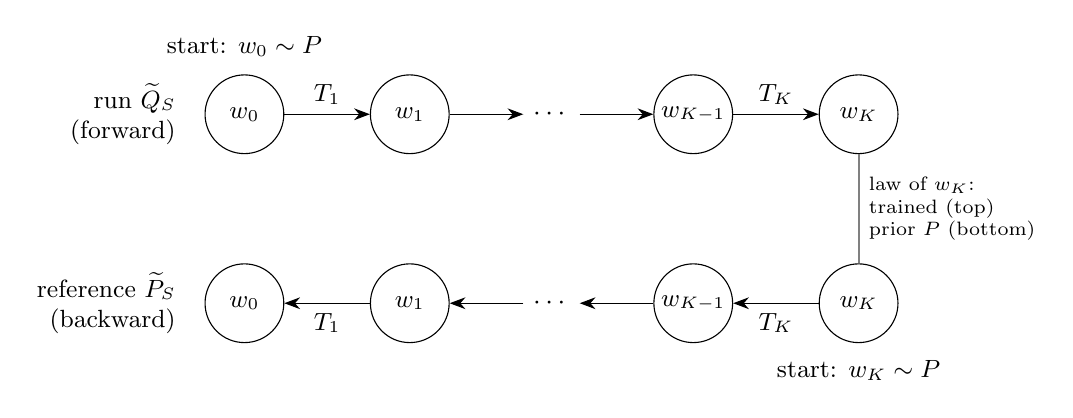
\begin{tikzpicture}[st/.style={circle,draw,minimum size=10mm,inner sep=0pt,font=\small}, >={Stealth[length=2mm]}]
\node[st] (a0) at (0,0) {$w_0$}; \node[st] (a1) at (2.1,0) {$w_1$}; \node (ad) at (3.9,0) {$\cdots$};
\node[st] (a3) at (5.7,0) {$w_{K-1}$}; \node[st] (a4) at (7.8,0) {$w_K$};
\node[st] (b0) at (0,-2.4) {$w_0$}; \node[st] (b1) at (2.1,-2.4) {$w_1$}; \node (bd) at (3.9,-2.4) {$\cdots$};
\node[st] (b3) at (5.7,-2.4) {$w_{K-1}$}; \node[st] (b4) at (7.8,-2.4) {$w_K$};
\draw[->] (a0) -- node[above]{\small $T_1$} (a1); \draw[->] (a1) -- (ad); \draw[->] (ad) -- (a3);
\draw[->] (a3) -- node[above]{\small $T_K$} (a4);
\draw[->] (b1) -- node[below]{\small $T_1$} (b0); \draw[->] (bd) -- (b1); \draw[->] (b3) -- (bd);
\draw[->] (b4) -- node[below]{\small $T_K$} (b3);
\node[above=1mm of a0, font=\small] {start: $w_0\sim P$}; \node[below=1mm of b4, font=\small] {start: $w_K\sim P$};
\node[anchor=east,align=right,font=\small] at (-0.75,0) {run $\Qt_S$\\ (forward)};
\node[anchor=east,align=right,font=\small] at (-0.75,-2.4) {reference $\Pt_S$\\ (backward)};
\draw[decorate,thick,gray] (a4.south) -- (b4.north) node[midway,right,align=left,font=\scriptsize,text=black] {law of $w_K$:\\ trained (top)\\ prior $P$ (bottom)};
\end{tikzpicture}
\caption{The two path distributions compared by the certificate. Their ratio $e^{C}$ is computable on the realised run
(Lemma~\ref{lem:path}). Because the reference has the data-free prior as its marginal at the output, PAC-Bayes can treat
it as a prior (Theorem~\ref{thm:cert}).}\label{fig:paths}
\end{figure}

\begin{assumption}[reversibility]\label{as:rev}
For every $S$ and $k$, $\gamma_k(\dd x)\,T_k(x,\dd y)=\gamma_k(\dd y)\,T_k(y,\dd x)$.
\end{assumption}
\begin{assumption}[what may depend on the data]\label{as:free}
The prior, the order of the examples and the stage boundaries are fixed independently of $S$. The kernels may depend on
$S$ and $k$ in any way (step sizes, mass matrices, even proposals computed from all of $S$), but are fixed before the run
starts: they may not adapt to the realised path. All maps $(S,x)\mapsto T_k^S(x,\cdot)$ are measurable.
\end{assumption}

\begin{lemma}[path identity]\label{lem:path}
Under Assumption~\ref{as:rev}, for every $S$, $\Qt_S=e^{C}\,\Pt_S$ as measures on $\mathcal{W}^{K+1}$, where
\[
C(w_{0:K})=\lambda\Big[\sum_{k=1}^K\ell_{B_k}(w_{k-1})-L_K(w_K)\Big].
\]
In particular $\Qt_S$ and $\Pt_S$ have the same null sets, and $\dd\Qt_S/\dd\Pt_S=e^{C}$.
\end{lemma}

\intuition{Reversibility says that, at equilibrium, a step of $T_k$ looks the same forwards and backwards. So the forward
and backward paths differ only in where they start and in which target each step is ``at equilibrium'' for. Walking
along the path, each time the target changes from $\gamma_{k-1}$ to $\gamma_k$ we pick up the ratio
$\gamma_{k-1}/\gamma_k=e^{\lambda\ell_{B_k}}$, evaluated at the state where the change happens, $w_{k-1}$. That gives the
prequential sum. At the end we pick up $\gamma_K/P=e^{-\lambda L_K}$ at $w_K$.}

\begin{proof}
Start from $\Qt_S$ and rewrite its first factor as $P(\dd w_0)=e^{\lambda\ell_{B_1}(w_0)}\gamma_1(\dd w_0)$, which holds
because $L_1=\ell_{B_1}$. Detailed balance for $T_1$ swaps the roles of $w_0$ and $w_1$:
$\gamma_1(\dd w_0)T_1(w_0,\dd w_1)=\gamma_1(\dd w_1)T_1(w_1,\dd w_0)$. Next,
$\gamma_1(\dd w_1)=e^{\lambda\ell_{B_2}(w_1)}\gamma_2(\dd w_1)$, and detailed balance for $T_2$ moves $\gamma_2$ from $w_1$ to
$w_2$. After $K$ such steps,
\[
\Qt_S(\dd w_{0:K})=e^{\lambda\sum_{k=1}^K\ell_{B_k}(w_{k-1})}\,\gamma_K(\dd w_K)\,T_K(w_K,\dd w_{K-1})\cdots T_1(w_1,\dd w_0),
\]
and finally $\gamma_K(\dd w_K)=e^{-\lambda L_K(w_K)}P(\dd w_K)$. Each step multiplies an identity between measures on two
coordinates by kernels and positive functions of the other coordinates, so it is an identity between measures on the
whole path. Only the measure form of detailed balance is used, so rejections (which put mass on staying put) need no
special treatment. Since $e^C$ is finite and positive, the two measures have the same null sets.
\end{proof}

\subsection{The certificate}
\begin{theorem}[certificate for the output network]\label{thm:cert}
Let $n\ge8$ and $\delta\in(0,1)$. Under Assumptions~\ref{as:rev} and~\ref{as:free}, with probability at least $1-\delta$
over the training set $S\sim D^n$ and the randomness of Algorithm~\ref{alg:ais},
\[
\kl\big(\err_S(w_K)\,\big\|\,\err_D(w_K)\big)\le\frac{C+\log(2\sqrt n/\delta)}{n},
\]
and hence $\err_D(w_K)\le\kl^{-1}\big(\err_S(w_K),\,(C+\log(2\sqrt n/\delta))/n\big)$.
\end{theorem}

\begin{proof}
Let $f_S(w)=\exp\big(n\,\kl(\err_S(w)\|\err_D(w))\big)$. For every fixed $w$, $\err_S(w)$ is an average of $n$ independent
Bernoulli variables, so $\E_S f_S(w)\le2\sqrt n$ (Maurer, 2004, Theorem~1). Consider $\varphi=f_S(w_K)e^{-C}$. By
Lemma~\ref{lem:path}, for every $S$,
\[
\E_{\Qt_S}[\varphi]=\int f_S(w_K)\,e^{-C}\,\dd\Qt_S=\int f_S(w_K)\,\dd\Pt_S=\E_{w\sim P}\big[f_S(w)\big].
\]
The last equality holds because $f_S(w_K)$ depends on the path only through $w_K$, and the $w_K$-marginal of $\Pt_S$ is $P$.
As $P$ does not depend on $S$, Tonelli's theorem lets us exchange the order of integration:
$\E_S\E_{\Qt_S}[\varphi]=\E_{w\sim P}\E_S[f_S(w)]\le2\sqrt n$. Markov's inequality over the joint draw of $S$ and the run
gives $\Prob(\varphi\ge2\sqrt n/\delta)\le\delta$, and on the complementary event
$n\,\kl(\err_S(w_K)\|\err_D(w_K))<C+\log(2\sqrt n/\delta)$.
\end{proof}

\review{A PAC-Bayes prior must not depend on the data, but $\Pt_S$ does, through the kernels. The proof uses $\Pt_S$ only to
integrate functions of $w_K$, whose law under $\Pt_S$ is the data-free $P$; the exchange of integrals is then over
$P\otimes D^n$. Please check that nothing else needs $\Pt_S$ to be data-free, and whether the measurability in
Assumption~\ref{as:free} suffices.}

\paragraph{Dictionary with standard PAC-Bayes.} The prior $P$ becomes the reference path measure $\Pt_S$, which is
data-free where it matters, at the output. The posterior $Q_S$ becomes the run's path measure $\Qt_S$. The log-density
ratio $\log\frac{\dd Q_S}{\dd P}(w)$ in (\ref{eq:disint}) becomes $C$, which, unlike the former, is computable.

\subsection{What is really needed, and why}\label{sec:whyrev}
\paragraph{Reversibility is sufficient, not necessary.} The proof of Lemma~\ref{lem:path} uses reversibility to write the
backward step of the reference $\Pt_S$ with the same kernel as the forward step of the run. Any invariant kernel would do, with its
\emph{time reversal} $T_k^\ast$ in the reference: the kernel defined by $\gamma_k(\dd x)T_k(x,\dd y)=\gamma_k(\dd y)T_k^\ast(y,\dd x)$,
which describes the forward chain run backwards at equilibrium and always exists for a $\gamma_k$-invariant $T_k$. The
telescoping, and hence $C$, is unchanged, and $T_k^\ast$ never has to be sampled, because the reference is never run.

\begin{remark}[general backward kernels]\label{rem:backward}
More generally still, the reference may use any backward kernels $R_k$:
$\Pt_S(\dd w_{0:K})=P(\dd w_K)\prod_kR_k(w_k,\dd w_{k-1})$ always has output marginal $P$, so Theorem~\ref{thm:cert} holds with
$C=\log\frac{P(w_0)}{P(w_K)}+\sum_k\log\frac{t_k(w_{k-1}\to w_k)}{r_k(w_k\to w_{k-1})}$ whenever these transition densities exist and
can be evaluated (this is the backward-kernel formalism of SMC samplers; Del Moral, Doucet and Jasra, 2006). Choosing
$R_k=T_k^\ast$ for invariant kernels gives our $C$.
\end{remark}

\paragraph{Why we choose reversible kernels anyway.}
\begin{enumerate}[nosep]
\item \textbf{Computability.} Reversibility turns intractable step probabilities into known loss differences; Lemma~\ref{lem:path}
  is this observation applied along the whole run.
\item \textbf{A reference that stays close to the run.} Run backwards from a prior sample with the same kernels, the
  reference looks like training played in reverse. The density ratio between the two processes, and hence $C$, is
  therefore small exactly when training goes well; with a poorly matched backward kernel the ratio would be large even
  for a good run.
\item \textbf{Tightness.} An invariant kernel actually targets the partial posterior $\pi_k$, so the network becomes an
  (approximate) posterior sample and Proposition~\ref{prop:intuition} applies: the price is the ideal KL plus Jensen gaps.
\item \textbf{Checkability.} For a reversible kernel the backward kernel is the training kernel itself, so reversibility
  can be tested directly: by running proposals forwards and backwards (Section~\ref{sec:exact}) and by the identity test of
  Section~\ref{sec:experiments}. HMC provides it for free.
\end{enumerate}

\subsection{What the posterior is, and how a classifier is drawn from it}\label{sec:posterior}
In standard PAC-Bayes one chooses a posterior family (say, Gaussians), fits its parameters, and then draws networks from
it. Here the order is reversed. The \emph{posterior} is, by definition, the distribution of the training run's output
given the data, $Q_S=\mathrm{law}(w_K\mid S)$, whatever that distribution turns out to be.
\begin{itemize}[nosep]
\item \textbf{Drawing a classifier} from $Q_S$ means running the training of Section~\ref{sec:training} once, with fresh
  randomness (initialisation, momenta, accept/reject coins). We certify that one network and then use it
  deterministically. Its training error $\err_S(w_K)$ is computed exactly; unlike certificates for stochastic
  classifiers, nothing has to be estimated by drawing many networks.
\item \textbf{Its density is never needed.} $Q_S$ has no closed form, and we never evaluate it: Lemma~\ref{lem:path}
  replaces the unknown ratio $\frac{\dd Q_S}{\dd P}(w_K)$ by the computable path ratio $e^C$, at the price of the extra term
  in Proposition~\ref{prop:kl}.
\item \textbf{Its shape.} $Q_S$ approximates the tempered posterior $\pi_K\propto e^{-\lambda L}P$, closely if the chain
  mixes well. That distribution is far from Gaussian: it is concentrated on regions of low training loss, with a width set
  by $\lambda$, and it is multimodal (every permutation of the hidden units gives an equivalent mode). At $\lambda=0.25$ it
  is ``warm'': sampled networks have training error $1.6\%$ on MNIST, where SGD would reach zero. It may sit far from the
  prior's centre in parameter space without any distance penalty, which is the main difference from Gaussian posteriors.
  Measuring its shape directly (for instance, the disagreement between networks from independent runs) is left for
  future work.
\end{itemize}

\subsection{What the complexity measures}
\begin{proposition}[the certificate pays at least the ideal price]\label{prop:kl}
\[\E_{\Qt_S}[C]=\KL(\Qt_S\|\Pt_S)\ge\KL\big(\mathrm{law}(w_K\mid S)\,\big\|\,P\big).\]
\end{proposition}
\begin{proof}
The equality restates Lemma~\ref{lem:path}. The inequality is the data-processing inequality for the map
$w_{0:K}\mapsto w_K$, which sends $\Qt_S$ to the law of the output and $\Pt_S$ to $P$.
\end{proof}
So, on average, the certificate is never better than the ordinary disintegrated bound with the same data-free prior and
the best possible posterior, the output's own law. The method does not beat the usual limits; it makes a bound on that
quantity computable. How far above the ideal is it? The cleanest case is a chain that mixes perfectly within each stage.

\begin{proposition}[perfect mixing: Gibbs KL plus Jensen gaps]\label{prop:intuition}
Suppose each $T_k$ returns an exact draw from $\pi_k$, independent of the past. Then $w_K\sim\pi_K$ and
\[
\E[C]=\KL(\pi_K\|P)+\sum_{k=1}^K J_k,\qquad
J_k=\lambda\,\E_{\pi_{k-1}}\big[\ell_{B_k}\big]+\log\E_{\pi_{k-1}}\big[e^{-\lambda\ell_{B_k}}\big]\ \ge0 .
\]
\end{proposition}
\begin{proof}
With perfect kernels $w_{k-1}\sim\pi_{k-1}$, so $\E[C]=\lambda\sum_k\E_{\pi_{k-1}}\ell_{B_k}-\lambda\E_{\pi_K}L_K$. On the
other hand $\KL(\pi_K\|P)=-\lambda\E_{\pi_K}L_K-\log Z_K$ and, as in (\ref{eq:preq}),
$-\log Z_K=\sum_k-\log\E_{\pi_{k-1}}e^{-\lambda\ell_{B_k}}$. Subtracting gives the identity, and $J_k\ge0$ by Jensen's
inequality.
\end{proof}

\intuition{$\KL(\pi_K\|P)$ is the complexity of the ideal Gibbs posterior (Section~\ref{sec:prequential}). The extra price
$J_k$ arises because a single network is charged the \emph{average} loss on block $k$ rather than the loss of the
posterior's averaged prediction; for small $\lambda\ell_{B_k}$ it is about $\frac{\lambda^2}{2}\mathrm{Var}_{\pi_{k-1}}(\ell_{B_k})$.
It is large when the posterior is still broad and the block is big, which is why the first blocks are small
($10,10,20,\dots$). Particles (Section~\ref{sec:smc}) shrink it further by charging the loss of a particle average. With
imperfect mixing Proposition~\ref{prop:kl} still holds.}

\paragraph{Is $C$ optimised?} No. Training samples the tempered posterior; it does not minimise $C$. The complexity is
\emph{measured} on the run, a by-product of training, much as a test error is measured rather than minimised. What we do
choose is the configuration (features, architecture, $\lambda$, stage sizes), by comparing certificates; Section~\ref{sec:select}
accounts for this choice. The main trade-off is $\lambda$: a larger $\lambda$ makes the posterior concentrate, so the
training error drops, but every block is charged more, so $C$ grows. Could one design kernels that drive $C$ down? Any
kernel that is reversible for $\gamma_k$ and fixed before the run is allowed, however clever, and a kernel that learns
faster from the first examples legitimately lowers $C$. What is not allowed is adapting the kernel along the run (for
example, tuning the step size from the acceptance rate), because then the steps are no longer draws from fixed kernels and
Lemma~\ref{lem:path} fails. No allowed choice can make the certificate invalid; at worst it makes it loose.

\begin{figure}[t]
\centering
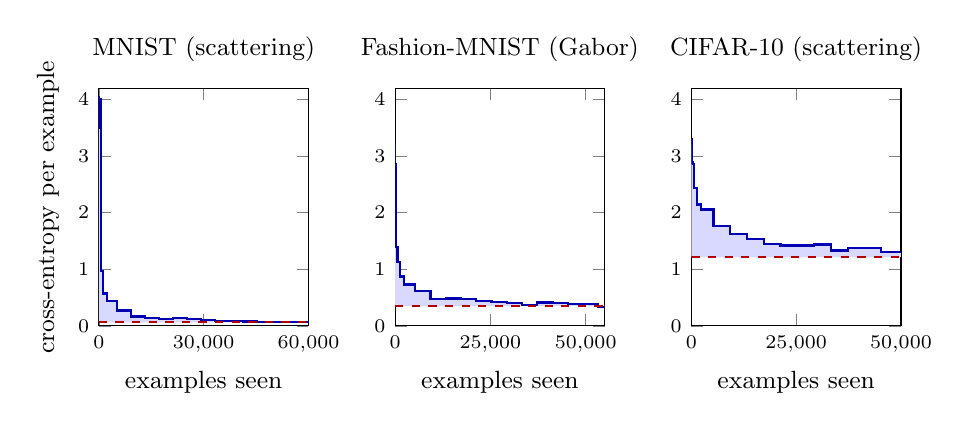
\begin{tikzpicture}
\begin{groupplot}[group style={group size=3 by 1, horizontal sep=1.1cm}, width=0.35\linewidth, height=4.6cm,
  xlabel={examples seen}, ymin=0, ymax=4.2, xmin=0, scaled x ticks=false, xticklabel style={/pgf/number format/fixed,font=\scriptsize},
  yticklabel style={font=\scriptsize}, title style={font=\small}, label style={font=\small}]
\nextgroupplot[title={MNIST (scattering)}, ylabel={cross-entropy per example}, xmax=60000, xtick={0,30000,60000}]
\addplot[name path=a, thick, blue!70!black, const plot] coordinates {(0,3.6484)(10,4.048)(20,3.8027)(40,3.829)(80,3.4982)(160,3.9425)(320,4.0015)(640,0.9751)(1280,0.5724)(2280,0.4329)(5280,0.2716)(9280,0.1657)(13280,0.1396)(17280,0.1215)(21280,0.1338)(25280,0.1144)(29280,0.0977)(33280,0.0869)(37280,0.0868)(41280,0.0782)(45280,0.0663)(49280,0.0673)(53280,0.0663)(57280,0.064)(60000,0.0602)};
\addplot[name path=b, thick, red!70!black, dashed] coordinates {(0,0.0619)(60000,0.0619)};
\addplot[blue!15] fill between[of=a and b];
\nextgroupplot[title={Fashion-MNIST (Gabor)}, xmax=55000, xtick={0,25000,50000}]
\addplot[name path=a, thick, blue!70!black, const plot] coordinates {(0,2.6204)(10,2.3432)(20,3.1955)(40,2.2864)(80,2.8608)(160,1.8938)(320,1.3982)(640,1.1255)(1280,0.8738)(2280,0.7314)(5280,0.6191)(9280,0.4804)(13280,0.4835)(17280,0.4787)(21280,0.4382)(25280,0.4222)(29280,0.4068)(33280,0.3728)(37280,0.4119)(41280,0.3981)(45280,0.3814)(49280,0.3817)(53280,0.3393)(55000,0.3613)};
\addplot[name path=b, thick, red!70!black, dashed] coordinates {(0,0.3534)(55000,0.3534)};
\addplot[blue!15] fill between[of=a and b];
\nextgroupplot[title={CIFAR-10 (scattering)}, xmax=50000, xtick={0,25000,50000}]
\addplot[name path=a, thick, blue!70!black, const plot] coordinates {(0,3.2017)(10,3.1267)(20,2.9467)(40,2.948)(80,3.2994)(160,2.8865)(320,2.8575)(640,2.4388)(1280,2.1436)(2280,2.0551)(5280,1.7702)(9280,1.6256)(13280,1.5326)(17280,1.4503)(21280,1.4194)(25280,1.4187)(29280,1.4382)(33280,1.3304)(37280,1.3709)(41280,1.3716)(45280,1.3077)(50000,1.3105)};
\addplot[name path=b, thick, red!70!black, dashed] coordinates {(0,1.2167)(50000,1.2167)};
\addplot[blue!15] fill between[of=a and b];
\end{groupplot}
\end{tikzpicture}
\caption{What the certificate pays. Solid: average cross-entropy on each new block, scored by the current network before
the chain uses it (a subset of the stages; $\lambda=0.25$). Dashed: final training cross-entropy. The shaded area, times
$\lambda$, is the complexity $C$; divided by $n$ it is the nats per example entering Theorem~\ref{thm:cert}. The axis is
linear, so the very lossy first blocks look thin, because they contain few examples. Models that learn quickly from
little data get small certificates.}\label{fig:curves}
\end{figure}

\subsection{How many blocks? The single-block limit and Gaussian PAC-Bayes}\label{sec:blocks}
\paragraph{The block sizes are a hyperparameter.} They may depend on $n$ but must be fixed before seeing the data
(Assumption~\ref{as:free}), and they count towards the selection budget (Section~\ref{sec:select}) like any other
choice. Proposition~\ref{prop:intuition} explains the trade-off. The price above the ideal is a sum of per-block Jensen
gaps, roughly $\frac{\lambda^2}2\mathrm{Var}_{\pi_{k-1}}(\ell_{B_k})$ each, which is large when a big block is scored while the
posterior is still broad. More and smaller blocks therefore lower the certificate, but every stage costs ten HMC moves
over all data seen so far. Our compromise is small blocks while the posterior is broad and blocks of $1{,}000$ later. On
MNIST pixels with $\lambda=1$, replacing uniform blocks of $1{,}000$ by this schedule lowered $C/n$ from $0.163$ to $0.140$
(certificate $0.217\to0.199$).

\paragraph{One block ($K=1$).} Then $C=\lambda[L(w_0)-L(w_K)]$: $\lambda$ times the training loss of a random
initialisation on all $n$ examples, minus the final training loss. The run is charged for the prior's ignorance on every
example at once, with no credit for learning along the way. With perfect mixing,
$\E[C]=\lambda\E_P[L]-\lambda\E_{\pi}[L]$, which is the realised version of the ``second-law'' bound of Harel et al.\
(2025), $\KL(\pi\|P)\le\lambda\E_P[L]$. A random initialisation has a cross-entropy of about $2$--$4$ nats per example in
our models, so $C/n\approx0.4$--$1.0$ and the certificate would be about $0.47$--$0.65$ on MNIST, $0.54$ on Fashion-MNIST and
$0.83$ on CIFAR-10, against $0.06$, $0.22$ and $0.61$ with the prequential schedule. (These are estimates from the
first stages of our runs, not separate runs.) The gain comes entirely from splitting the data so that each block is
charged after the network has learned from the previous ones.

\paragraph{Relation to Gaussian PAC-Bayes (P\'erez-Ortiz et al.).} No choice of blocks reduces the method to the
Gaussian setting. Both use a data-free Gaussian prior and the same PAC-Bayes theorem, but they differ in the posterior and
in how its price is computed:
\begin{center}\small
\renewcommand{\arraystretch}{1.2}
\begin{tabular}{@{}p{3.0cm}p{6.0cm}p{5.6cm}@{}}
\toprule
 & Gaussian PAC-Bayes & this note\\
\midrule
posterior & $N(\mu,\Sigma)$, $\mu$ near SGD weights, $\Sigma$ learned & law of the output of an MCMC run\\
how it is fitted & minimise the bound over $(\mu,\Sigma)$ by gradient descent & it is not fitted; it is what training produces\\
complexity & closed-form $\KL(N(\mu,\Sigma)\,\|\,P)$ & realised path ratio $C$\\
what it charges & distance from initialisation; precision of $\Sigma$ & online loss minus final loss\\
classifier certified & random draws (Gibbs classifier), risk estimated by sampling & one deterministic network\\
\bottomrule
\end{tabular}
\end{center}
The Gaussian approach can be tight when the trained weights are close to the initialisation relative to the prior's
scale; ours is tight when the model learns quickly from few examples, wherever in parameter space it ends up.

\subsection{Other annealing paths: invariances and temperature}\label{sec:paths}
The proof of Lemma~\ref{lem:path} used only that $\gamma_0=P$ and that each $T_k$ is reversible for its $\gamma_k$; the
specific form of $\gamma_k$ played no role.

\begin{corollary}[general annealing paths]\label{cor:general}
Let $\gamma_k=e^{-U_k}P$ for any functions $U_1,\dots,U_K$ (possibly depending on $S$), $U_0\equiv0$, with each $T_k$
reversible for $\gamma_k$. Then Theorem~\ref{thm:cert} holds with
$C=\sum_{k=1}^K\big(U_k-U_{k-1}\big)(w_{k-1})-U_K(w_K)$.
\end{corollary}
\begin{proof}
Repeat the proof of Lemma~\ref{lem:path} with $\gamma_{k-1}=e^{U_k-U_{k-1}}\gamma_k$.
\end{proof}
Three instances:
\begin{enumerate}[nosep]
\item \emph{Data path} (this note): $U_k=\lambda L_k$.
\item \emph{Built-in invariances (augmentation)}: $U_k(w)=\lambda\sum_{i\le n_k}\frac1{|G|}\sum_{g\in G}\ell(w,gz_i)$ for a fixed,
  data-free set $G$ of transformations, for example the identity and a horizontal flip. The certificate still concerns the
  0-1 error on untransformed data; $G$ only shapes the posterior.
\item \emph{Temperature path}: $U_k=\beta_kL$ with $0=\beta_0<\dots<\beta_K$, giving
  $C=\sum_k(\beta_k-\beta_{k-1})L(w_{k-1})-\beta_KL(w_K)$. With perfect mixing and vanishing increments this tends to
  $\int_0^{\beta}\E_{\pi_b}L\,\dd b-\beta L(w_K)$, the temperature integral of Maurer, Mirzaei and Pontil (2025);
  Corollary~\ref{cor:general} certifies the realised, finite-step version of their quantity. The data path charges each
  example once, while the temperature path charges every example at every temperature. Which is tighter in practice is
  an open experiment.
\end{enumerate}

\subsection{Choosing among configurations}\label{sec:select}
Hyperparameters (features, $\lambda$, architecture) are compared by their certificates on the same training set. If $G$
configurations are tried, applying Theorem~\ref{thm:cert} to each with $\delta/G$ makes all bounds hold simultaneously.
We fix $G=100$ per dataset in advance and count every full-data run ever made. At $n=60{,}000$ this adds
$\log(100)/n\approx8\cdot10^{-5}$ nats per example, which changes no reported digit beyond the fourth decimal. Seeds are
never selected: every seed run is reported.

\subsection{Particles}\label{sec:smc}
Running $P$ chains in parallel and resampling them at each stage according to how well they predicted the new block
(sequential Monte Carlo) gives a certificate for one of the final particles with $C=-\lambda L_K(w_{\text{out}})-\log\hat Z$,
where $-\log\hat Z=-\sum_k\log\frac1P\sum_m e^{-\lambda\ell_{B_k}(w^{m}_{k-1})}$ is $\lambda$ times the online log-loss of
the particle average. With one particle this is the $C$ above. The proof uses the particle-Gibbs construction of Andrieu,
Doucet and Holenstein (2010) and is in Appendix~\ref{app:smc}. In our experiments $8$ particles reduce $C$ by at most
$3\%$, so the main results use single chains.

%======================================================================
\section{Exactness: why floating point breaks the certificate, and a fix}\label{sec:exact}

\paragraph{The problem.} Lemma~\ref{lem:path} requires each kernel to be \emph{exactly} reversible. On a computer the
state space is a finite set of floating-point vectors, and a standard HMC implementation violates reversibility in three
ways: the leapfrog integrator is not exactly time-reversible under rounding, Gaussian random numbers are not exactly
Gaussian, and the Metropolis test uses a rounded exponential.

\begin{example}[why no small correction suffices]
Suppose rounding makes the proposal map send two different states $a\neq a'$ to the same state $b$. A forward step
$a\to b$ then has positive probability, but the reversed step from $b$ can return to only one of $a,a'$. Some forward
paths therefore have probability zero under the reference $\Pt_S$, and on those paths the true log-ratio is $+\infty$,
not $C$ plus a small error.
\end{example}

The same issue is known in differential privacy, which also rests on exact probability ratios: floating-point Laplace
noise was broken in practice (Mironov, 2012), and the floating-point Gaussian noise of DP-SGD libraries was attacked with
up to $93\%$ success (Jin et al., 2022). The accepted fix there is exact discrete sampling (Canonne, Kamath and Steinke,
2020). The same caveat applies to every certificate that samples noise in floating point, including Gaussian PAC-Bayes
posteriors and priors obtained by private training.

\paragraph{The fix: HMC on integer lattices.} Keep every random choice and every acceptance decision exact, and let
floating-point arithmetic only \emph{propose} moves. That is harmless as long as the proposal map is an exact bijection
that is its own inverse.
\begin{itemize}[nosep]
\item Weights and momenta live on integer lattices: $w=2^{-24}\,i$ with $i\in\Z^d$, and momenta $j\in\Z^d$.
\item The prior is a \emph{discrete Gaussian} on the lattice, and momenta are drawn from a discrete Gaussian with integer
  variance. Both are sampled exactly with integer arithmetic (Canonne et al., 2020).
\item The target at stage $k$ is defined by whatever the computer returns for the block losses:
  $\pi_k(i)\propto P(i)\exp(-\lambda\sum_{b\le k}\hat\ell_b(i))$, where $\hat\ell_b(i)$ is the floating-point number
  computed by one fixed routine. Any deterministic function is allowed, because it simply \emph{defines} the target, and
  the same numbers enter $C$. All energies are then exact rational numbers.
\item The leapfrog steps become integer ``shears'': $j\leftarrow j-\rint(\tau\hat g(i)/\epsilon)$ and
  $i\leftarrow i+\rint(c\,j)$, where $\hat g$ is the floating-point gradient and $\rint$ rounds to the nearest integer. A
  shear is undone exactly by subtracting the same integer, whatever $\hat g$ computes, so the integrator followed by a
  momentum flip is an exact involution (bit-reversible dynamics; Levesque and Verlet, 1993).
\item The Metropolis test uses an exact Bernoulli$(e^{-\gamma})$ sampler for the exact rational $\gamma$.
\end{itemize}
The remaining assumptions are ideal random bits, as in all MCMC and differential-privacy work, and determinism: the
computer must return the same bits for the same weights. Determinism is audited during every run, by recomputing earlier
block losses bit for bit at each stage and by explicitly running proposals forwards and then backwards.
Appendix~\ref{app:exact} gives the details and the proof (Proposition~\ref{prop:exact}). The exact sampler runs at the
same speed as the floating-point one, and the headline numbers below use it where available.

%======================================================================
\section{Experiments}\label{sec:experiments}

\subsection{Setup}
\begin{itemize}[nosep]
\item \textbf{Data.} MNIST ($n=60{,}000$), Fashion-MNIST ($n=55{,}000$, the training file used throughout this project,
  not standardised with training statistics), CIFAR-10 ($n=50{,}000$); ten classes; the standard test sets of
  $10{,}000$ images, used only for reporting; $\delta=0.025$.
\item \textbf{Data-free features.} Fixed filters, no learning. \emph{Gabor} features (a first-order scattering transform):
  8 orientations $\times$ 2 scales of complex Gabor filters, the modulus of each response, average-pooled over $4\times4$
  blocks, plus a pooled copy of the image ($833$ features for $28\times28$ images; applied per colour channel for
  CIFAR). \emph{Scattering} features add second-order terms, the fine-scale moduli filtered again by the coarse filters
  (Bruna and Mallat, 2013; $3{,}969$ features for $28\times28$ images, $15{,}552$ for CIFAR). Each example's feature
  vector is standardised using only that example's own mean and standard deviation.
\item \textbf{Model.} A one-hidden-layer MLP (100 ReLU units) on the features; prior $N(0,2/\text{fan-in})$ for weights,
  $N(0,0.1)$ for biases.
\item \textbf{Sampler.} $\lambda=0.25$; the stages above; $10$ HMC moves of $50$ leapfrog steps per stage; step size
  $1.5/\sqrt{1+\lambda\max(n_k,300)}$, a fixed function of the stage. A full run takes 40--110 minutes on CPU or GPU.
\end{itemize}

\subsection{Is the bound valid? Tests that would catch mistakes}
Theorem~\ref{thm:cert} rests on Lemma~\ref{lem:path}, which predicts something checkable: reweighting runs by $e^{-C}$ must
reproduce the prior, $\E_{\Qt_S}[e^{-C}g(w_K)]=\E_{w\sim P}[g(w)]$ for every $g\ge0$, and in particular $\E[e^{-C}]=1$. We
test this by brute force on a tiny network (a 2-4-3 MLP, $n=8$, three stages) with $2\cdot10^6$ runs, including two
deliberately broken variants. Heavy-tailed weights bias the sample mean down, which is the safe direction; an error that
makes $C$ too optimistic shows up as values \emph{above} the prior's.

\begin{center}\small
\begin{tabular}{@{}lccc@{}}
\toprule
variant & $\E[e^{-C}]$ (target 1) & reweighted loss (target 1.503) & verdict\\
\midrule
AIS, floating point & 0.993--0.998 & 1.477--1.494 & passes\\
SMC (4 particles), floating point & 0.993 & 1.474 & passes\\
AIS, exact lattice, $5\cdot10^5$ runs & $1.003\pm0.007$ & $1.509\pm0.023$ & passes\\
broken: Metropolis test removed & $1.60$ ($z=15$) & 3.62 & caught\\
broken: block scored after training & $1.08$ ($z=64$) & 1.39 & caught\\
\bottomrule
\end{tabular}
\end{center}
The second broken variant is the most natural implementation mistake: it makes the online loss look smaller than it is,
and the test detects it at once. In the exact runs, $30{,}090$ explicit forward-backward round trips and every
determinism audit passed.

On real data, a valid certificate can never fall below the true error. Over 120 runs on random MNIST subsets of
$1{,}000$ examples (true and random labels, $\lambda\in\{0.25,1,4\}$, 20 seeds each) it never fell below the test error.
With random labels, where every classifier has true error $0.9$, the certificate was always at least $0.949$, including at
$\lambda=4$, where the network fits a third of the noise and $C$ grows to compensate. At full size the random-label
certificate is $0.924$.

\subsection{Results}
\begin{table}[h]
\centering\small
\begin{tabular}{@{}llcccc@{}}
\toprule
data & model & train error & test error & $C/n$ & \textbf{certificate}\\
\midrule
MNIST & scattering + MLP, exact, 2 seeds & 0.016 / 0.016 & 0.015 / 0.015 & 0.024 & \textbf{0.060 / 0.060}\\
MNIST & Gabor + MLP, exact, 2 seeds & 0.023 / 0.023 & 0.021 / 0.021 & 0.024 & 0.073 / 0.072\\
MNIST & MLP on pixels (floating point) & 0.037 & 0.043 & 0.083 & 0.167\\
Fashion & scattering + MLP, exact & 0.114 & 0.119 & 0.036 & \textbf{0.217}\\
Fashion & Gabor + MLP, exact & 0.122 & 0.126 & 0.032 & 0.221\\
CIFAR-10 & scattering + MLP (floating point) & 0.422 & 0.441 & 0.073 & \textbf{0.612}\\
CIFAR-10 & Gabor + MLP (floating point) & 0.455 & 0.464 & 0.060 & 0.626\\
\bottomrule
\end{tabular}
\caption{Certificates from Algorithm~\ref{alg:ais} ($\lambda=0.25$, $\delta=0.025$). Adjusting for selection among 100
configurations changes them by at most $0.0002$. The Fashion scattering configuration was fixed in advance from the MNIST
choice.}\label{tab:results}
\end{table}

\begin{table}[h]
\centering\small
\begin{tabular}{@{}lccc@{}}
\toprule
data-free certificate, full training set & MNIST & Fashion & CIFAR-10\\
\midrule
P\'erez-Ortiz et al.\ (2021), Gaussian PAC-Bayes & 0.217 (CNN) & -- & --\\
Garc\'ia-P\'erez et al.\ (2025), Gaussian PAC-Bayes & 0.315 & -- & 0.738\\
Lotfi et al.\ (2022), compression & 0.116 & -- & --\\
Lampert et al.\ (2026), prior from private training & 0.233 & -- & 0.716\\
ours, DP-SGD + mutual information (earlier) & 0.070 & 0.249 & 0.715\\
\textbf{ours, this note} & \textbf{0.060} & \textbf{0.217} & \textbf{0.612}\\
\bottomrule
\end{tabular}
\caption{Comparison, with published numbers as reported by the papers. Results that learn the prior on part of the data
(e.g.\ $0.016$ on MNIST by P\'erez-Ortiz et al.) are not comparable and are omitted.}\label{tab:compare}
\end{table}

\paragraph{Where the remaining slack is.} The certificate is roughly the training error plus a term that grows like
$\sqrt{\text{train error}\times C/n}$. On MNIST both are small. On Fashion-MNIST and CIFAR-10 the training error of the
sampled network dominates ($0.11$ of $0.22$, and $0.42$ of $0.61$): the tempered posterior on data-free features does not
fit these datasets well. Gains must therefore come from models that fit better while keeping the online loss low, using
data-free ingredients only, such as better invariances (Corollary~\ref{cor:general}, item 2) and better features. More
compute per stage does not help: twenty times more HMC moves left the online loss unchanged.

%======================================================================
\section{Related work}\label{sec:related}
\paragraph{PAC-Bayes certificates for networks.} Gaussian posteriors with data-free priors (Dziugaite and Roy, 2017;
P\'erez-Ortiz et al., 2021; Garc\'ia-P\'erez et al., 2025) pay for the distance travelled by SGD and for the posterior's
shape; we replace the Gaussian by an MCMC-approximated Gibbs posterior and pay its learning curve. Compression bounds
(Lotfi et al., 2022) pay a description length of the weights; ours is a prequential description length of the data given
the model. Data-dependent priors built by differentially private training (Dziugaite and Roy, 2018; Lampert,
Cairney-Leeming and Zakerinia, 2026) pay the information leaked by noisy training.
\paragraph{Gibbs posteriors and Langevin dynamics.} Gibbs posteriors minimise PAC-Bayes objectives (Catoni, 2007), and
PAC-Bayes and the Bayesian marginal likelihood are closely related (Germain et al., 2016). Closest to us, Maurer, Mirzaei
and Pontil (2025) bound a draw from the exact Gibbs posterior using a temperature integral of the expected training loss,
estimated along a Langevin chain and calibrated on random labels, on binary versions of MNIST and CIFAR-10; Harel et al.\
(2025) bound Markov training processes by a second-law argument. Our bound holds for the actual output of a finite run,
without mixing assumptions or estimated expectations, and the temperature integral is a special case of
Corollary~\ref{cor:general}.
\paragraph{Learning speed and generalisation.} Prequential code lengths explain the generalisation of deep networks
(Blier and Ollivier, 2018), and training speed estimates the marginal likelihood (Lyle et al., 2020). Excess Description
Length (2026) studies the prequential-minus-final quantity in expectation. We turn this intuition into a
high-probability certificate for a specific network.
\paragraph{Annealing and path-space ratios.} The path identity is that of AIS (Neal, 2001) and Jarzynski's equality
(Jarzynski, 1997; Crooks, 1998), in the backward-kernel form of SMC samplers (Del Moral, Doucet and Jasra, 2006). The same
log-weights bound KL divergences to the posterior in bidirectional Monte Carlo (Grosse, Ghahramani and Adams, 2015;
Grosse, Ancha and Roy, 2016).
\paragraph{Exactness.} Bit-reversible integrators come from molecular dynamics (Levesque and Verlet, 1993); exact discrete
Gaussian sampling and the floating-point concern come from differential privacy (Mironov, 2012; Canonne, Kamath and
Steinke, 2020; Jin et al., 2022). We are not aware of their use to make a generalisation certificate exact.
\paragraph{What appears to be new.} (i) Using the realised path log-ratio of an annealed run as the complexity of a
disintegrated PAC-Bayes bound, with a data-dependent reference whose output marginal is data-free; (ii) the data path,
which charges each point once; (iii) the exact implementation; (iv) the resulting numbers. These claims rest on quick
literature searches and need a thorough one.

%======================================================================
\section{Limitations and open questions}
\begin{itemize}[nosep]
\item \textbf{The certified network is trained by MCMC, not SGD.} It reaches test errors of $1.5\%$ (MNIST), $12\%$
  (Fashion-MNIST) and $44\%$ (CIFAR-10). Explaining SGD-trained networks needs a bridge, for instance an SGD solution used
  as a proposal inside a reversible kernel, which Assumption~\ref{as:free} allows.
\item \textbf{Data-free features carry much of the result.} On pixels the MNIST certificate is $0.167$.
\item \textbf{Cost.} Each run costs about $30{,}000$ full-data gradient evaluations.
\item \textbf{Open experiments.} Data versus temperature paths; invariances (horizontal flips, results pending); an exact
  version of the particle method.
\end{itemize}

%======================================================================
\appendix
\section{Proof for the particle method}\label{app:smc}
\begin{algorithm}[h]
\caption{Particle version (\texttt{--P} $>1$)}\label{alg:smc}
\begin{algorithmic}[1]
\State draw $x_0^1,\dots,x_0^P\sim P$ independently
\For{$k=1,\dots,K$}
  \State weights $W_k^m\propto G_k(x_{k-1}^m)$ with $G_k=\gamma_k/\gamma_{k-1}=e^{-\lambda\ell_{B_k}}$; \ $\hat Z_k=\frac1P\sum_mG_k(x_{k-1}^m)$
  \State for $j=1..P$: draw an ancestor $a_k^j\sim\mathrm{Categorical}(W_k)$, then $x_k^j\sim T_k(x_{k-1}^{a_k^j},\cdot)$
\EndFor
\State draw $b$ uniformly from $\{1,\dots,P\}$; output $x_K^b$ with $C=-\lambda L_K(x_K^b)-\log\hat Z$, $\hat Z=\prod_k\hat Z_k$
\end{algorithmic}
\end{algorithm}

\begin{proposition}\label{prop:smc}
Theorem~\ref{thm:cert} holds for the output $x_K^b$ of Algorithm~\ref{alg:smc}, with $C=-\lambda L_K(x_K^b)-\log\hat Z$.
\end{proposition}
\begin{proof}
Write $\xi$ for all particles and ancestor indices. The law of $(\xi,b)$ is
\[
\Qt(\xi,b)=\tfrac1P\textstyle\prod_jP(\dd x_0^j)\prod_{k}\prod_jW_k^{a_k^j}\,T_k(x_{k-1}^{a_k^j},\dd x_k^j).
\]
Trace the output back through its ancestors: $b_K=b$ and $b_{k-1}=a_k^{b_k}$. Let $\rho$ be the path measure
$\rho(\dd x_{0:K})=Z_K^{-1}P(\dd x_0)\prod_kG_k(x_{k-1})T_k(x_{k-1},\dd x_k)$. Its final marginal is $\pi_K$, by induction:
$PG_1=\gamma_1$, $T_k$ leaves $\gamma_k$ invariant, and $\gamma_kG_{k+1}=\gamma_{k+1}$. The conditional-SMC target of
Andrieu, Doucet and Holenstein (2010) is
\[
\tilde\pi(\xi,b)=P^{-(K+1)}\rho\big(\dd x_{0:K}^{b_{0:K}}\big)\textstyle\prod_{j\ne b_0}P(\dd x_0^j)\prod_k\prod_{j\ne b_k}W_k^{a_k^j}\,T_k(x_{k-1}^{a_k^j},\dd x_k^j).
\]
It is a probability measure (the lineage indices $(b_0,\dots,b_K)$ range bijectively over $\{1..P\}^{K+1}$, $\rho$ has mass
one, and the remaining factors are conditional laws), and its output $x_K^b$ has law $\pi_K$. In $\Qt/\tilde\pi$ every factor
off the lineage cancels, leaving
\[
\frac{\Qt}{\tilde\pi}=P^KZ_K\prod_k\frac{W_k^{b_{k-1}}}{G_k(x_{k-1}^{b_{k-1}})}=\frac{Z_K}{\hat Z},
\]
because $W_k^m/G_k(x_{k-1}^m)=1/\sum_{m'}G_k(x_{k-1}^{m'})$. Set $\Pt=\tilde\pi\cdot\frac{\dd P}{\dd\pi_K}(x_K^b)$, a probability
measure whose output marginal is $P$. Then
$\frac{\dd\Qt}{\dd\Pt}=\frac{Z_K}{\hat Z}\frac{\dd\pi_K}{\dd P}(x_K^b)=\frac{e^{-\lambda L_K(x_K^b)}}{\hat Z}=e^{C}$, and the proof of
Theorem~\ref{thm:cert} applies with $x_K^b$ in place of $w_K$.
\end{proof}
The code returns slot $1$ instead of a uniformly drawn $b$. After multinomial resampling and independent moves the final
particles are exchangeable, and $\hat Z$ does not depend on their labels, so this changes nothing.

\section{The exact lattice sampler}\label{app:exact}
Fix the lattice spacing $\Delta=2^{-24}$ and, for each group $g$ of parameters (a weight matrix or a bias vector), the
prior variance $v_g\in\mathbb{Q}$.
\begin{itemize}[nosep]
\item \emph{State:} $(i,j)\in\Z^d\times\Z^d$; weights $w=\Delta i$, exactly representable in float64; momenta
  $p_g=\epsilon_gj$ with $\epsilon_g=(v_gN)^{-1/2}$ and $N=2^{24}$.
\item \emph{Prior:} $P(i)\propto\prod_d\exp(-i_d^2/(2s_g^2))$ with $s_g^2=v_g/\Delta^2$, sampled exactly (Canonne et al.,
  2020, Algorithm~3, with big integers).
\item \emph{Momentum:} $\mu(j)\propto\prod_d\exp(-j_d^2/(2N))$, sampled exactly in 64-bit integers; kinetic energy
  $\kappa(j)=\sum_dj_d^2/(2N)$.
\item \emph{Targets:} $\pi_k(i)\propto P(i)\exp(-\lambda\sum_{b\le k}\hat\ell_b(i))$, where $\hat\ell_b(i)$ is computed by a
  single forward pass over block $b$ and an exactly rounded sum. The energies
  $E_k(i)=\sum_di_d^2/(2s_g^2)+\lambda\sum_{b\le k}\hat\ell_b(i)$ are exact rationals.
\item \emph{Proposal:} the shears $A_\tau(i,j)=(i,\,j-\rint(\tau\hat g(i)/\epsilon))$ and $B_\tau(i,j)=(i+\rint(c_\tau j),\,j)$ with
  $c_\tau=\tau v\epsilon/\Delta$, composed palindromically, $\Phi=A_{h/2}B_hA_h\cdots A_hB_hA_{h/2}$, then the flip
  $F(i,j)=(i,-j)$.
\item \emph{Acceptance} with probability $\min\{1,e^{\Delta H}\}$, $\Delta H=E_k(i)+\kappa(j)-E_k(i')-\kappa(j')\in\mathbb{Q}$, by an exact
  Bernoulli$(e^{-\gamma})$ sampler (Canonne et al., 2020, Algorithm~1).
\item \emph{One move:} draw $j\sim\mu$, propose $(i',j')=F\Phi(i,j)$, accept or stay, discard the momentum. $T_k$ is ten
  moves.
\end{itemize}

\begin{proposition}\label{prop:exact}
If $\hat g$ and $\hat\ell_b$ are deterministic functions of $i$ and the random bits are ideal, then each $T_k$ is exactly
reversible with respect to $\pi_k$, $w_0$ has law exactly $P$, and $C=\lambda[\sum_k\hat\ell_k(i_{k-1})-\sum_b\hat\ell_b(i_K)]$
is an exact rational. Theorem~\ref{thm:cert} therefore holds for the lattice network $\Delta i_K$, as the computer
evaluates it.
\end{proposition}
\begin{proof}
\emph{The proposal is an exact involution.} Each shear is a bijection of $\Z^{2d}$, undone by subtracting the same
integer, for any deterministic $\hat g$, accurate or not. Rounding to nearest (ties to even) and floating-point
multiplication are odd functions, so $FB_\tau F=B_\tau^{-1}$; and $FA_\tau F=A_\tau^{-1}$ because the increment of $A_\tau$
depends only on $i$. For the palindromic $\Phi$ this gives $F\Phi F=\Phi^{-1}$, that is, $(F\Phi)^2=\mathrm{id}$.

\emph{The Metropolis step is reversible on $\Z^{2d}$} with respect to $\pi_k\otimes\mu$: for a deterministic involutive
proposal on a countable space the usual argument applies with counting measure, with no Jacobian, and the acceptance
probability is realised exactly.

\emph{The move is reversible on positions alone.} For $i\neq i'$,
\[
\pi_k(i)\,T(i,i')=\sum_{j:\,(F\Phi(i,j))_1=i'}\pi_k(i)\,\mu(j)\,\alpha\big((i,j),F\Phi(i,j)\big).
\]
The map $j\mapsto j'=(F\Phi(i,j))_2$ is a
bijection from $\{j:(F\Phi(i,j))_1=i'\}$ onto $\{j':(F\Phi(i',j'))_1=i\}$, its inverse being the same formula because $F\Phi$ is
an involution. Detailed balance on $\Z^{2d}$ turns each term into $\pi_k(i')\mu(j')\alpha((i',j'),(i,j))$, and summing over $j'$
gives $\pi_k(i')T(i',i)$. A composition of such moves is reversible as well.

\emph{The rest.} $w_0$ is an exact discrete Gaussian draw, and $C$ uses the same $\hat\ell_b$ as the targets, so it
telescopes exactly in rational arithmetic. It is rounded upward before use.
\end{proof}

\section{Checklist for the reviewer}\label{sec:checklist}
\begin{enumerate}[nosep]
\item Theorem~\ref{thm:cert}: is using the data-dependent reference $\Pt_S$ only through its output marginal enough? Are
  further measurability conditions needed?
\item Lemma~\ref{lem:path}: the telescoping as an identity of measures, including rejections; and its extension to
  invariant (not necessarily reversible) kernels via time reversals, and to general backward kernels
  (Section~\ref{sec:whyrev}, Remark~\ref{rem:backward}).
\item Proposition~\ref{prop:hmc}: reversibility of the HMC move (shears, involution, detailed balance on the extended space,
  and the passage to the weight kernel).
\item Proposition~\ref{prop:intuition}: the perfect-mixing decomposition and the reading of $J_k$.
\item Proposition~\ref{prop:smc}: the conditional-SMC target for resample-then-move, and outputting slot 1.
\item Proposition~\ref{prop:exact}: odd symmetry of rounding and of floating-point multiplication; the passage from a
  reversible step on $\Z^{2d}$ to a reversible kernel on positions.
\item Data-freeness: prior, features (fixed filters, per-example standardisation), pixel scaling, order, stage boundaries.
\item The step size depends only on the stage; nothing adapts to the path.
\item Selection: about 27 full-data configurations on MNIST, 6 on Fashion-MNIST and 5 on CIFAR-10 so far, within the
  declared budget of 100 each; seeds are never selected.
\end{enumerate}

\begin{thebibliography}{99}\small
\bibitem{adh} C.~Andrieu, A.~Doucet, R.~Holenstein. Particle Markov chain Monte Carlo methods. \emph{JRSS-B}, 2010.
\bibitem{bf} G.~Blanchard, F.~Fleuret. Occam's hammer. \emph{COLT}, 2007.
\bibitem{bo} L.~Blier, Y.~Ollivier. The description length of deep learning models. \emph{NeurIPS}, 2018.
\bibitem{bm} J.~Bruna, S.~Mallat. Invariant scattering convolution networks. \emph{IEEE TPAMI}, 2013.
\bibitem{cks} C.~Canonne, G.~Kamath, T.~Steinke. The discrete Gaussian for differential privacy. \emph{NeurIPS}, 2020.
\bibitem{catoni} O.~Catoni. \emph{PAC-Bayesian supervised classification: the thermodynamics of statistical learning}. IMS, 2007.
\bibitem{crooks} G.~Crooks. Nonequilibrium measurements of free energy differences for microscopically reversible Markovian systems. \emph{J.\ Stat.\ Phys.}, 1998.
\bibitem{dawid} A.~P.~Dawid. Present position and potential developments: the prequential approach. \emph{JRSS-A}, 1984.
\bibitem{ddj} P.~Del Moral, A.~Doucet, A.~Jasra. Sequential Monte Carlo samplers. \emph{JRSS-B}, 2006.
\bibitem{dr17} G.~K.~Dziugaite, D.~M.~Roy. Computing nonvacuous generalization bounds for deep (stochastic) neural networks with many more parameters than training data. \emph{UAI}, 2017.
\bibitem{dr18} G.~K.~Dziugaite, D.~M.~Roy. Data-dependent PAC-Bayes priors via differential privacy. \emph{NeurIPS}, 2018.
\bibitem{edl} Excess Description Length. arXiv:2601.04728, 2026.
\bibitem{gp} Garc\'ia-P\'erez et al. Data-free PAC-Bayes certificates for neural networks, 2025 (see \texttt{docs/literature.md}).
\bibitem{germain} P.~Germain, F.~Bach, A.~Lacoste, S.~Lacoste-Julien. PAC-Bayesian theory meets Bayesian inference. \emph{NeurIPS}, 2016.
\bibitem{grosse15} R.~Grosse, Z.~Ghahramani, R.~Adams. Sandwiching the marginal likelihood using bidirectional Monte Carlo. arXiv:1511.02543, 2015.
\bibitem{grosse16} R.~Grosse, S.~Ancha, D.~Roy. Measuring the reliability of MCMC inference with bidirectional Monte Carlo. \emph{NeurIPS}, 2016.
\bibitem{harel} I.~Harel, Y.~Wolanowsky, G.~Vardi, N.~Srebro, D.~Soudry. Temperature is all you need for generalization in Langevin dynamics and other Markov processes. arXiv:2505.19087, 2025.
\bibitem{jarz} C.~Jarzynski. Nonequilibrium equality for free energy differences. \emph{Phys.\ Rev.\ Lett.}, 1997.
\bibitem{jin} J.~Jin, E.~McMurtry, B.~Rubinstein, O.~Ohrimenko. Are we there yet? Timing and floating-point attacks on differential privacy systems. \emph{IEEE S\&P}, 2022.
\bibitem{lz} C.~H.~Lampert, J.~Cairney-Leeming, N.~Zakerinia. arXiv:2605.26222, v2, 2026.
\bibitem{lv} D.~Levesque, L.~Verlet. Molecular dynamics and time reversibility. \emph{J.\ Stat.\ Phys.}, 1993.
\bibitem{lotfi} S.~Lotfi et al. PAC-Bayes compression bounds so tight that they can explain generalization. \emph{NeurIPS}, 2022.
\bibitem{lyle} C.~Lyle, L.~Schut, B.~Ru, Y.~Gal, M.~van der Wilk. A Bayesian perspective on training speed and model selection. \emph{NeurIPS}, 2020.
\bibitem{maurer} A.~Maurer. A note on the PAC Bayesian theorem. arXiv:cs/0411099, 2004.
\bibitem{mmp} A.~Maurer, E.~Mirzaei, M.~Pontil. Generalization of Gibbs and Langevin Monte Carlo algorithms in the interpolation regime. arXiv:2510.06028, 2025.
\bibitem{mironov} I.~Mironov. On significance of the least significant bits for differential privacy. \emph{CCS}, 2012.
\bibitem{neal} R.~Neal. Annealed importance sampling. \emph{Statistics and Computing}, 2001.
\bibitem{neal11} R.~Neal. MCMC using Hamiltonian dynamics. \emph{Handbook of Markov Chain Monte Carlo}, 2011.
\bibitem{po} M.~P\'erez-Ortiz, O.~Rivasplata, J.~Shawe-Taylor, C.~Szepesv\'ari. Tighter risk certificates for neural networks. \emph{JMLR}, 2021.
\bibitem{riva} O.~Rivasplata, I.~Kuzborskij, C.~Szepesv\'ari, J.~Shawe-Taylor. PAC-Bayes analysis beyond the usual bounds. \emph{NeurIPS}, 2020.
\bibitem{seeger} M.~Seeger. PAC-Bayesian generalisation error bounds for Gaussian process classification. \emph{JMLR}, 2002.
\bibitem{viallard} P.~Viallard, R.~Emonet, A.~Habrard, E.~Morvant, V.~Zantedeschi. Leveraging PAC-Bayes theory and Gibbs distributions for generalization bounds with complexity measures. \emph{AISTATS}, 2024.
\end{thebibliography}
\end{document}
